\PassOptionsToPackage{unicode=true}{hyperref} % options for packages loaded elsewhere
\PassOptionsToPackage{hyphens}{url}
%
\documentclass[]{article}
\usepackage{lmodern}
\usepackage{amssymb,amsmath}
\usepackage{ifxetex,ifluatex}
\usepackage{fixltx2e} % provides \textsubscript
\ifnum 0\ifxetex 1\fi\ifluatex 1\fi=0 % if pdftex
  \usepackage[T1]{fontenc}
  \usepackage[utf8]{inputenc}
  \usepackage{textcomp} % provides euro and other symbols
\else % if luatex or xelatex
  \usepackage{unicode-math}
  \defaultfontfeatures{Ligatures=TeX,Scale=MatchLowercase}
\fi
% use upquote if available, for straight quotes in verbatim environments
\IfFileExists{upquote.sty}{\usepackage{upquote}}{}
% use microtype if available
\IfFileExists{microtype.sty}{%
\usepackage[]{microtype}
\UseMicrotypeSet[protrusion]{basicmath} % disable protrusion for tt fonts
}{}
\IfFileExists{parskip.sty}{%
\usepackage{parskip}
}{% else
\setlength{\parindent}{0pt}
\setlength{\parskip}{6pt plus 2pt minus 1pt}
}
\usepackage{hyperref}
\hypersetup{
            pdftitle={Ellipsoid Method and Its Amazing Oracles},
            pdfauthor={Wai-Shing Luk},
            pdfkeywords={Ellipsoid method, Cutting plane method, Separation oracle, Cholesky Factorization},
            pdfborder={0 0 0},
            breaklinks=true}
\urlstyle{same}  % don't use monospace font for urls
\usepackage{listings}
\newcommand{\passthrough}[1]{#1}
\usepackage{graphicx,grffile}
\makeatletter
\def\maxwidth{\ifdim\Gin@nat@width>\linewidth\linewidth\else\Gin@nat@width\fi}
\def\maxheight{\ifdim\Gin@nat@height>\textheight\textheight\else\Gin@nat@height\fi}
\makeatother
% Scale images if necessary, so that they will not overflow the page
% margins by default, and it is still possible to overwrite the defaults
% using explicit options in \includegraphics[width, height, ...]{}
\setkeys{Gin}{width=\maxwidth,height=\maxheight,keepaspectratio}
\setlength{\emergencystretch}{3em}  % prevent overfull lines
\providecommand{\tightlist}{%
  \setlength{\itemsep}{0pt}\setlength{\parskip}{0pt}}
\setcounter{secnumdepth}{5}
% Redefines (sub)paragraphs to behave more like sections
\ifx\paragraph\undefined\else
\let\oldparagraph\paragraph
\renewcommand{\paragraph}[1]{\oldparagraph{#1}\mbox{}}
\fi
\ifx\subparagraph\undefined\else
\let\oldsubparagraph\subparagraph
\renewcommand{\subparagraph}[1]{\oldsubparagraph{#1}\mbox{}}
\fi

% set default figure placement to htbp
\makeatletter
\def\fps@figure{htbp}
\makeatother

\ifxetex \usepackage[UTF8]{ctex} \fi
\usepackage{tikz,pgf,pgfplots}
\usetikzlibrary{arrows}
\definecolor{qqqqff}{rgb}{0.,0.,1.}
\newcommand{\columnsbegin}{}
\newcommand{\columnsend}{}
\newcommand{\col}[1]{}
\newcommand{\pause}{}
\newcommand{\onslide}{}

\title{Ellipsoid Method and Its Amazing Oracles\thanks{This work was supported by the Society for Industrial and Applied
Mathematics}}
\author{Wai-Shing Luk\thanks{Fudan University}}
\date{\today}

\begin{document}
\maketitle
\begin{abstract}
Ellipsoid method is revisited. Besides that, three separation oracles
are investigated for applications. They are robust optimization,
semidefinite programming, and network optimization. Discuss stability
issue. Finally, the parallel cut is described.
\end{abstract}

\hypertarget{introduction}{%
\section{Introduction}\label{introduction}}

The bad reputation of the ellipsoid method is not good. And that is
unfair. It is commonly believed that the method is inefficient in
practice for large-scale convex problems. The convergent rate is slow.
It cannot exploits sparsity. It was supplanted by the interior-point
methods. It can be treated as a theoretical tool for proving the
polynomial-time solvability of combinatorial optimization problems.

However, the ellipsoid method works very differently compared with the
interior point method. it only requires a separation oracle. Thus, it
can play nicely with other techniques. Consider Ellipsoid Method When
the number of optimization variables is moderate, e.g.~ECO flow, analog
circuit sizing, parametric problems. The number of constraints is large,
or even infinite. Whenever separation oracle can be implemented
efficiently.

\hypertarget{cutting-plane-method-revisited}{%
\section{Cutting-plane Method
Revisited}\label{cutting-plane-method-revisited}}

\hypertarget{convex-feasibility-problem}{%
\subsection{Convex Feasibility
Problem}\label{convex-feasibility-problem}}

Let \(\mathcal{K} \subseteq \mathbb{R}^n\) be a convex set. Consider the
feasibility problem:

\begin{itemize}
\tightlist
\item
  Find a point \(x^* \in \mathbb{R}^n\) in \(\mathcal{K}\),
\item
  or determine that \(\mathcal{K}\) is empty (i.e., no feasible
  solution)
\end{itemize}

\begin{figure}
\hypertarget{fig:region}{%
\centering

\includegraphics{ellipsoid.files/region.pdf}
\caption{Feasibility region}\label{fig:region}
}
\end{figure}

When a \emph{separation oracle} \(\Omega\) is \emph{queried} at \(x_0\),
it either

\begin{itemize}
\tightlist
\item
  asserts that \(x_0 \in \mathcal{K}\), or
\item
  returns a separating hyperplane between \(x_0\) and \(\mathcal{K}\):
\end{itemize}

\[g^\top (x - x_0) + \beta \leq 0, \beta \geq 0, g \neq 0, \; \forall x \in \mathcal{K}\]
\{\#eq:cut\}

\begin{figure}
\hypertarget{fig:cut}{%
\centering
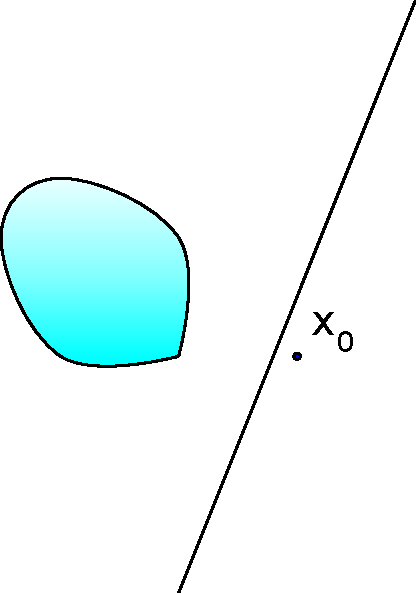
\includegraphics{ellipsoid.files/cut.pdf}
\caption{Cut}\label{fig:cut}
}
\end{figure}

The pair \((g, h)\) is called a \emph{cutting-plane}, or cut, since it
eliminates the halfspace \(\{x \mid g^\top (x - x_0) + h > 0\}\) from
our search. If \(h=0\) (\(x_0\) is on the boundary of halfspace that is
cut), cutting-plane is called \emph{neutral cut}. If \(h>0\) (\(x_0\)
lies in the interior of halfspace that is cut), cutting-plane is called
\emph{deep cut}.

The \(\mathcal{K}\) is usually given by a set of inequalities
\(f_j(x) \le 0\) or \(f_j(x) < 0\) for \(j = 1 \cdots m\), where
\(f_j(x)\) is a convex function. A vector \(g \equiv \partial f(x_0)\)
is called a \emph{subgradient} of a convex function \(f\) at \(x_0\) if
\(f(z) \geq f(x_0) + g^\mathrm{T} (z - x_0)\). Hence, the cut \((g, h)\)
is given by \((\partial f(x_0), f(x_0))\)

Note that if \(f(x)\) is differentiable, we can simply take
\(\partial f(x_0) = \nabla f(x_0)\)

Cutting-plane method consists of two key components: separation oracle
\(\Omega\) and a search space \(\mathcal{S}\) initially big enough to
cover \(\mathcal{K}\). For example,

\begin{itemize}
\tightlist
\item
  Polyhedron \(\mathcal{P}\) = \(\{z \mid C z \preceq d \}\)
\item
  Interval \(\mathcal{I}\) = \([l, u]\) (for one-dimensional problem)
\item
  Ellipsoid \(\mathcal{E}\) =
  \(\{z \mid (z-x_c)P^{-1}(z-x_c) \leq 1 \}\)
\end{itemize}

Generic Cutting-plane method:

\begin{itemize}
\tightlist
\item
  \textbf{Given} initial \(\mathcal{S}\) known to contain
  \(\mathcal{K}\).
\item
  \textbf{Repeat}

  \begin{enumerate}
  \def\labelenumi{\arabic{enumi}.}
  \tightlist
  \item
    Choose a point \(x_0\) in \(\mathcal{S}\)
  \item
    Query the cutting-plane oracle at \(x_0\)
  \item
    \textbf{If} \(x_0 \in \mathcal{K}\), quit
  \item
    \textbf{Else}, update \(\mathcal{S}\) to a smaller set that covers:
    \[\mathcal{S}^+ = \mathcal{S} \cap \{z \mid g^\top (z - x_0) + h \leq 0\}\]
  \item
    \textbf{If} \(\mathcal{S}^+ = \emptyset\) or it is small enough,
    quit.
  \end{enumerate}
\end{itemize}

Listing: Feasibility Code

\begin{lstlisting}[language=Python, label=lst:feasibility_code]
def cutting_plane_feas(evaluate, S, options=Options()):
    feasible = False
    status = 0
    for niter in range(options.max_it):
        cut, feasible = evaluate(S.xc)
        if feasible:  # feasible sol'n obtained
            break
        status, tsq = S.update(cut)
        if status != 0:
            break
        if tsq < options.tol:
            status = 2
            break
    return S.xc, niter+1, feasible, status
\end{lstlisting}

\hypertarget{convex-optimization-problem}{%
\subsection{Convex Optimization
Problem}\label{convex-optimization-problem}}

Consider:

\[\begin{array}{ll}
    \text{minimize}     & f_0(x), \\
    \text{subject to}   & x \in \mathcal{K}
\end{array}\] \{\#eq:convex\_optimization\}

The optimization problem is treated as a feasibility problem with an
additional constraint \(f_0(x) < t\). Here, \(f_0(x)\) could be a convex
function or a quasiconvex function. \(t\) is the best-so-far value of
\(f_0(x)\). The problem can be reformulated as:

\[\begin{array}{ll}
    \text{minimize}     & t, \\
    \text{subject to}   & \Phi(x, t) < 0 \\
                        & x \in \mathcal{K}
\end{array}\] \{\#eq:cvx\_in\_feasibility\_form\}

where \(\Phi(x, t) < 0\) is the \(t\)-sublevel set of \(f_0(x)\). Note
that \(\mathcal{K}_t \subseteq \mathcal{K}_u\) if and only if
\(t \leq u\) (monotonicity). One easy way to solve the optimization
problem is to apply the binary search on \(t\).

Listing: Binary search

\begin{lstlisting}[language=Python, label=lst:binary_search]
def bsearch(evaluate, I, options=Options()):
    feasible = False
    l, u = I
    t = l + (u - l)/2
    for niter in range(options.max_it):
        if evaluate(t):  # feasible sol'n obtained
            feasible = True
            u = t
        else:
            l = t
        tau = (u - l)/2
        t = l + tau
        if tau < options.tol:
            break
    return u, niter+1, feasible
\end{lstlisting}

\begin{lstlisting}[language=Python]
class bsearch_adaptor:
    def __init__(self, P, E, options=Options()):
        self.P = P
        self.E = E
        self.options = options

    @property
    def x_best(self):
        return self.E.xc

    def __call__(self, t):
        E = self.E.copy()
        self.P.update(t)
        x, _, feasible, _ = cutting_plane_feas(
            self.P, E, self.options)
        if feasible:
            self.E._xc = x.copy()
            return True
        return False
\end{lstlisting}

\hypertarget{shrinking}{%
\subsection{Shrinking}\label{shrinking}}

\begin{itemize}
\tightlist
\item
  Another possible way is, to update the best-so-far \(t\) whenever a
  feasible solution \(x_0\) is found such that \(\Phi(x_0, t) = 0\).
\item
  We assume that the oracle takes the responsibility for that.
\end{itemize}

\hypertarget{generic-cutting-plane-method-optim}{%
\subsection{Generic Cutting-plane method
(Optim)}\label{generic-cutting-plane-method-optim}}

\begin{itemize}
\tightlist
\item
  \textbf{Given} initial \(\mathcal{S}\) known to contain
  \(\mathcal{K}_t\).
\item
  \textbf{Repeat}

  \begin{enumerate}
  \def\labelenumi{\arabic{enumi}.}
  \tightlist
  \item
    Choose a point \(x_0\) in \(\mathcal{S}\)
  \item
    Query the separation oracle at \(x_0\)
  \item
    \textbf{If} \(x_0 \in \mathcal{K}_t\), update \(t\) such that
    \(\Phi(x_0, t) = 0\).
  \item
    Update \(\mathcal{S}\) to a smaller set that covers:
    \[\mathcal{S}^+ = \mathcal{S} \cap \{z \mid g^\top (z - x_0) + h \leq 0\} \]
  \item
    \textbf{If} \(\mathcal{S}^+ = \emptyset\) or it is small enough,
    quit.
  \end{enumerate}
\end{itemize}

\hypertarget{corresponding-python-code}{%
\subsection{Corresponding Python code}\label{corresponding-python-code}}

\begin{lstlisting}[language=Python]
def cutting_plane_dc(evaluate, S, t, options=Options()):
    feasible = False  # no sol'n
    x_best = S.xc
    for niter in range(options.max_it):
        cut, t1 = evaluate(S.xc, t)
        if t != t1:  # best t obtained
            feasible = True
            t = t1
            x_best = S.xc
        status, tau = S.update(cut)
        if status == 1:
            break
        if tau < options.tol:
            status = 2
            break
    return x_best, t, niter+1, feasible, status
\end{lstlisting}

\hypertarget{example-profit-maximization-problem}{%
\subsection{Example: Profit Maximization
Problem}\label{example-profit-maximization-problem}}

\[\begin{array}{ll}
   \text{maximize} & p(A x_1^\alpha x_2^\beta) - v_1 x_1 - v_2 x_2 \\
   \text{subject to}& x_1 \le k.
\end{array}\]

\begin{itemize}
\tightlist
\item
  \(p(A x_1^\alpha x_2^\beta)\) : Cobb-Douglas production function
\item
  \(p\): the market price per unit
\item
  \(A\): the scale of production
\item
  \(\alpha, \beta\): the output elasticities
\item
  \(x\): input quantity
\item
  \(v\): output price
\item
  \(k\): a given constant that restricts the quantity of \(x_1\)
\end{itemize}

\hypertarget{example-profit-maximization-contd}{%
\subsection{Example: Profit maximization
(cont'd)}\label{example-profit-maximization-contd}}

\begin{itemize}
\tightlist
\item
  The formulation is not in the convex form.
\item
  Rewrite the problem in the following form: \[\begin{array}{ll}
    \text{maximize} & t \\
    \text{subject to} & t  + v_1 x_1  + v_2 x_2 < p A x_1^{\alpha} x_2^{\beta}\\
                  & x_1 \le k.
    \end{array}\]
\end{itemize}

\hypertarget{profit-maximization-in-convex-form}{%
\subsection{Profit maximization in Convex
Form}\label{profit-maximization-in-convex-form}}

\begin{itemize}
\item
  By taking the logarithm of each variable:

  \begin{itemize}
  \tightlist
  \item
    \(y_1 = \log x_1\), \(y_2 = \log x_2\).
  \end{itemize}
\item
  We have the problem in a convex form:
\end{itemize}

\[\begin{array}{ll}
    \text{max}  & t \\
    \text{s.t.} & \log(t + v_1 e^{y_1} + v_2 e^{y_2}) - (\alpha y_1 + \beta y_2) < \log(pA) \\
                & y_1 \le \log k.
\end{array}\]

\hypertarget{python-code-profit-oracle}{%
\subsection{Python code (Profit
oracle)}\label{python-code-profit-oracle}}

\scriptsize

\begin{lstlisting}[language=Python]
class profit_oracle:
    def __init__(self, params, a, v):
        p, A, k = params
        self.log_pA = np.log(p * A)
        self.log_k = np.log(k)
        self.v = v
        self.a = a

    def __call__(self, y, t):
        fj = y[0] - self.log_k  # constraint
        if fj > 0.:
            g = np.array([1., 0.])
            return (g, fj), t
        log_Cobb = self.log_pA + np.dot(self.a, y)
        x = np.exp(y)
        vx = np.dot(self.v, x)
        te = t + vx
        fj = np.log(te) - log_Cobb
        if fj < 0.:
            te = np.exp(log_Cobb)
            t = te - vx
            fj = 0.
        g = (self.v * x) / te - self.a
        return (g, fj), t
\end{lstlisting}

\hypertarget{python-code-main-program}{%
\subsection{Python code (Main program)}\label{python-code-main-program}}

\begin{lstlisting}[language=Python]
import numpy as np
from profit_oracle import *
from cutting_plane import *
from ell import *

p, A, k = 20.0, 40.0, 30.5
params = p, A, k
a = np.array([0.1, 0.4])
v = np.array([10.0, 35.0])
y0 = np.array([0., 0.])  # initial x0
E = ell(200, y0)
P = profit_oracle(params, a, v)
yb1, fb, niter, feasible, status = \
    cutting_plane_dc(P, E, 0.0)
print(fb, niter, feasible, status)
\end{lstlisting}

\hypertarget{area-of-applications}{%
\subsection{Area of Applications}\label{area-of-applications}}

\begin{itemize}
\tightlist
\item
  Robust convex optimization

  \begin{itemize}
  \tightlist
  \item
    oracle technique: affine arithmetic
  \end{itemize}
\item
  Parametric network potential problem

  \begin{itemize}
  \tightlist
  \item
    oracle technique: negative cycle detection
  \end{itemize}
\item
  Semidefinite programming

  \begin{itemize}
  \tightlist
  \item
    oracle technique: Cholesky factorization
  \end{itemize}
\end{itemize}

\hypertarget{robust-convex-optimization}{%
\section{Robust Convex Optimization}\label{robust-convex-optimization}}

\hypertarget{robust-optimization-formulation}{%
\subsection{Robust Optimization
Formulation}\label{robust-optimization-formulation}}

\begin{itemize}
\item
  Consider: \[\begin{array}{ll}
      \text{minimize}   & \sup_{q \in \mathbb Q} f_0(x,q) \\
      \text{subject to} & f_j(x,q) \leq 0, \;
       \forall q \in {\mathbb Q}, \; j = 1,2,\cdots,m,
    \end{array}\] where \(q\) represents a set of varying parameters.
\item
  The problem can be reformulated as: \[\begin{array}{ll}
      \text{minimize}   & t \\
      \text{subject to} & f_0(x,q) < t  \\
      & f_j(x,q) \leq 0, \;
       \forall q \in {\mathbb Q}, \; j = 1,2,\cdots,m,
    \end{array}\]
\end{itemize}

\hypertarget{oracle-in-robust-optimization-formulation}{%
\subsection{Oracle in Robust Optimization
Formulation}\label{oracle-in-robust-optimization-formulation}}

\begin{itemize}
\tightlist
\item
  The oracle only needs to determine:

  \begin{itemize}
  \tightlist
  \item
    If \(f_j(x_0, q) > 0\) for some \(j\) and \(q = q_0\), then

    \begin{itemize}
    \tightlist
    \item
      the cut \((g, h)\) = \((\partial f_j(x_0, q_0), f_j(x_0, q_0))\)
    \end{itemize}
  \item
    If \(f_0(x_0, q) \geq t\) for some \(q = q_0\), then

    \begin{itemize}
    \tightlist
    \item
      the cut \((g, h)\) =
      \((\partial f_0(x_0, q_0), f_0(x_0, q_0) - t)\)
    \end{itemize}
  \item
    Otherwise, \(x_0\) is feasible, then

    \begin{itemize}
    \tightlist
    \item
      Let \(q_{\max} = \text{argmax}_{q \in \mathbb Q} f_0(x_0, q)\).
    \item
      \(t := f_0(x_0, q_{\max})\).
    \item
      The cut \((g, h)\) = \((\partial f_0(x_0, q_{\max}), 0)\)
    \end{itemize}
  \end{itemize}
\item
  Random sampling trick
\end{itemize}

\hypertarget{example-profit-maximization-problem-convex}{%
\subsection{Example: Profit Maximization Problem
(convex)}\label{example-profit-maximization-problem-convex}}

\[\begin{array}{ll}
\text{max}  & t \\
\text{s.t.} & \log(t + \hat{v}_1 e^{y_1} + \hat{v}_2 e^{y_2}) - (\hat{\alpha} y_1 + \hat{\beta} y_2) \le \log(\hat{p}\,A)  \\
                  & y_1 \le \log \hat{k} ,
\end{array}\]

\begin{itemize}
\tightlist
\item
  Now assume that:

  \begin{itemize}
  \tightlist
  \item
    \(\hat{\alpha}\) and \(\hat{\beta}\) vary \(\bar{\alpha} \pm e_1\)
    and \(\bar{\beta} \pm e_2\) respectively.
  \item
    \(\hat{p}\), \(\hat{k}\), \(\hat{v}_1\), and \(\hat{v}_2\) all vary
    \(\pm e_3\).
  \end{itemize}
\end{itemize}

\hypertarget{example-profit-maximization-problem-oracle}{%
\subsection{Example: Profit Maximization Problem
(oracle)}\label{example-profit-maximization-problem-oracle}}

By detail analysis, the worst case happens when:

\begin{itemize}
\tightlist
\item
  \(p = \bar{p} + e_3\), \(k = \bar{k} + e_3\)
\item
  \(v_1 = \bar{v}_1 - e_3\), \(v_2 = \bar{v}_2 - e_3\),
\item
  if \(y_1 > 0\), \(\alpha = \bar{\alpha} - e_1\), else
  \(\alpha = \bar{\alpha} + e_1\)
\item
  if \(y_2 > 0\), \(\beta = \bar{\beta} - e_2\), else
  \(\beta = \bar{\beta} + e_2\)
\end{itemize}

\begin{quote}
\textbf{Remark}: for more complicated problems, affine arithmetic could
be used.
\end{quote}

\hypertarget{profit_rb_oracle}{%
\subsection{\texorpdfstring{\texttt{profit\_rb\_oracle}}{profit\_rb\_oracle}}\label{profit_rb_oracle}}

\begin{lstlisting}[language=Python]
class profit_rb_oracle:
    def __init__(self, params, a, v, vparams):
        ui, e1, e2, e3 = vparams
        self.uie = [ui * e1, ui * e2]
        self.a = a
        p, A, k = params
        p -= ui * e3
        k -= ui * e3
        v_rb = v.copy()
        v_rb += ui * e3
        self.P = profit_oracle((p, A, k), a, v_rb)

    def __call__(self, y, t):
        a_rb = self.a.copy()
        for i in [0, 1]:
            a_rb[i] += self.uie[i] if y[i] <= 0. \
                              else -self.uie[i]
        self.P.a = a_rb
        return self.P(y, t)
\end{lstlisting}

\hypertarget{parametric-network-potential-problem}{%
\section{Parametric Network Potential
Problem}\label{parametric-network-potential-problem}}

\hypertarget{parametric-network-potential-problem-1}{%
\subsection{Parametric Network Potential
Problem}\label{parametric-network-potential-problem-1}}

Given a network represented by a directed graph \(G = (V, E)\).

Consider:

\[\begin{array}{ll}
    \text{minimize} & t \\
    \text{subject to} & u_i - u_j \le h_{ij}(x, t), \; \forall (i, j) \in E ,\\
    \text{variables} &x, u ,
   \end{array}\]

\begin{itemize}
\item
  \(h_{ij}(x, t)\) is the weight function of edge \((i,j)\),
\item
  Assume: network is large but the number of parameters is small.
\end{itemize}

\hypertarget{network-potential-problem-contd}{%
\subsection{Network Potential Problem
(cont'd)}\label{network-potential-problem-contd}}

Given \(x\) and \(t\), the problem has a feasible solution if and only
if \(G\) contains no negative cycle. Let \(\mathcal{C}\) be a set of all
cycles of \(G\).

\[\begin{array}{ll}
    \text{minimize} & t \\
    \text{subject to} & W_k(x, t) \ge 0, \forall C_k \in C ,\\
       \text{variables} & x
   \end{array}\]

\begin{itemize}
\item
  \(C_k\) is a cycle of \(G\)
\item
  \(W_k(x, t) = \sum_{ (i,j)\in C_k} h_{ij}(x, t)\).
\end{itemize}

\hypertarget{oracle-in-network-potential-problem}{%
\subsection{Oracle in Network Potential
Problem}\label{oracle-in-network-potential-problem}}

\begin{itemize}
\tightlist
\item
  The oracle only needs to determine:

  \begin{itemize}
  \tightlist
  \item
    If there exists a negative cycle \(C_k\) under \(x_0\), then

    \begin{itemize}
    \tightlist
    \item
      the cut \((g, h)\) = \((-\partial W_k(x_0), -W_k(x_0))\)
    \end{itemize}
  \item
    If \(f_0(x_0) \geq t\), then

    \begin{itemize}
    \tightlist
    \item
      the cut \((g, h)\) = \((\partial f_0(x_0), f_0(x_0) - t)\)
    \end{itemize}
  \item
    Otherwise, \(x_0\) is feasible, then

    \begin{itemize}
    \tightlist
    \item
      \(t := f_0(x_0)\).
    \item
      The cut \((g, h)\) = \((\partial f_0(x_0), 0)\)
    \end{itemize}
  \end{itemize}
\end{itemize}

\hypertarget{python-code}{%
\subsection{Python Code}\label{python-code}}

\begin{lstlisting}[language=Python]
class network_oracle:
    def __init__(self, G, f, p):
        self.G = G
        self.f = f
        self.p = p  # partial derivative of f w.r.t x
        self.S = negCycleFinder(G)

    def __call__(self, x):
        def get_weight(G, e):
            return self.f(G, e, x)

        self.S.get_weight = get_weight
        C = self.S.find_neg_cycle()
        if C is None:
            return None, 1
        f = -sum(self.f(self.G, e, x) for e in C)
        g = -sum(self.p(self.G, e, x) for e in C)
        return (g, f), 0
\end{lstlisting}

\hypertarget{example-optimal-matrix-scaling}{%
\subsection{Example: Optimal Matrix
Scaling}\label{example-optimal-matrix-scaling}}

\begin{itemize}
\item
  Given a sparse matrix \(A = [a_{ij}] \in \mathbb{R}^{N\times N}\).
\item
  Find another matrix \(B = U A U^{-1}\) where \(U\) is a nonnegative
  diagonal matrix, such that the ratio of any two elements of \(B\) in
  absolute value is as close to 1 as possible.
\item
  Let \(U = \mathrm{diag}([u_1, u_2, \ldots, u_N])\). Under the
  min-max-ratio criterion, the problem can be formulated as:
\end{itemize}

\[\begin{array}{ll}
  \text{minimize}   &   \pi/\psi  \\
  \text{subject to} &   \psi \leq u_i |a_{ij}| u_j^{-1} \leq \pi, \; \forall a_{ij} \neq 0 , \\
                    &   \pi, \, \psi, u, \text{positive} \\
  \text{variables}  &   \pi, \psi, u \, .
  \end{array}\]

\hypertarget{optimal-matrix-scaling-contd}{%
\subsection{Optimal Matrix Scaling
(cont'd)}\label{optimal-matrix-scaling-contd}}

By taking the logarithms of variables, the above problem can be
transformed into:

\[\begin{array}{ll}
  \text{minimize}   &   t \\
  \text{subject to} &   \pi' - \psi' \leq t \\
                    &   u_i' - u_j'  \leq \pi' - a_{ij}', \; \forall a_{ij} \neq 0 \,, \\
                    &   u_j' - u_i' \leq a_{ij}' - \psi', \; \forall a_{ij} \neq 0 \,, \\
  \text{variables}  &   \pi', \psi', u' \, .
  \end{array}\]

where \(k'\) denotes \(\log( | k | )\) and \(x = (\pi', \psi' )^\top\).

\hypertarget{corresponding-python-code-1}{%
\subsection{Corresponding Python
Code}\label{corresponding-python-code-1}}

\scriptsize

\begin{lstlisting}[language=Python]
def constr(G, e, x):
    u, v = e
    i_u = G.node_idx[u]
    i_v = G.node_idx[v]
    cost = G[u][v]['cost']
    return x[0] - cost if i_u <= i_v else cost - x[1]

def pconstr(G, e, x):
    u, v = e
    i_u = G.node_idx[u]
    i_v = G.node_idx[v]
    return np.array([1.,  0.] if i_u <= i_v else [0., -1.])

class optscaling_oracle:
    def __init__(self, G):
        self.network = network_oracle(G, constr, pconstr)

    def __call__(self, x, t):
        cut, feasible = self.network(x)
        if not feasible: return cut, t
        s = x[0] - x[1]
        fj = s - t
        if fj < 0.:
            t = s
            fj = 0.
        return (np.array([1., -1.]), fj), t
\end{lstlisting}

\hypertarget{example-clock-period-yield-driven-co-optimization}{%
\subsection{Example: clock period \& yield-driven
co-optimization}\label{example-clock-period-yield-driven-co-optimization}}

\[\begin{array}{cll}
   \text{minimize} &T_{CP} - w_\beta \beta \\
   \text{subject to} & u_i - u_j \le T_{CP} + F_{ij}^{-1}(1 - \beta), & \forall (i,j) \in E_s \,,\\
                     & u_j - u_i \le F_{ij}^{-1}(1 - \beta), & \forall (j,i) \in E_h \,, \\
                     & T_{CP} \ge 0, \, 0 \le \beta \le 1 \, , \\
    \text{variables} &T_{CP}, \beta, u.
   \end{array}\]

\begin{itemize}
\tightlist
\item
  Note that \(F_{ij}^{-1}(x)\) is not concave in general in \([0, 1]\).
\item
  Fortunately, we are most likely interested in optimizing circuits for
  high yield rather than the low one in practice.
\item
  Therefore, by imposing an additional constraint to \(\beta\), say
  \(\beta \geq 0.8\), the problem becomes convex.
\end{itemize}

\hypertarget{inverse-cdf}{%
\subsection{Inverse CDF}\label{inverse-cdf}}

\begin{figure}
\centering
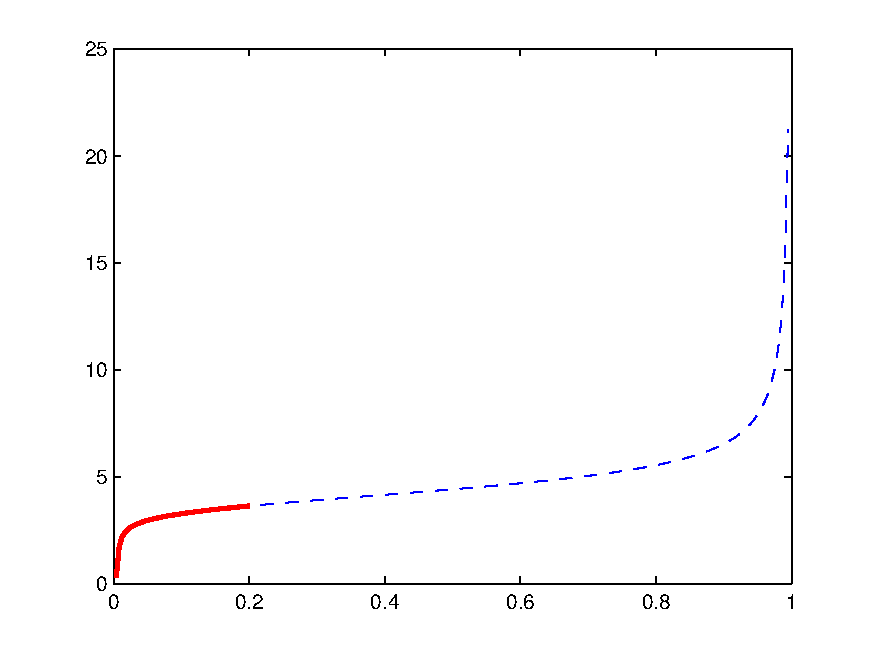
\includegraphics{ellipsoid.files/Fig2-b-invcdf.pdf}
\caption{img}
\end{figure}

\hypertarget{matrix-inequalities}{%
\section{Matrix Inequalities}\label{matrix-inequalities}}

\hypertarget{problems-with-matrix-inequalities}{%
\subsection{Problems With Matrix
Inequalities}\label{problems-with-matrix-inequalities}}

Consider the following problem:

\[\begin{array}{ll}
    \text{minimize}    & t, \\
    \text{subject to}  & F(x, t) \succeq 0,
\end{array}\]

\begin{itemize}
\tightlist
\item
  \(F(x, t)\): a matrix-valued function
\item
  \(A \succeq 0\) denotes \(A\) is positive semidefinite.
\end{itemize}

\hypertarget{problems-with-matrix-inequalities-1}{%
\subsection{Problems With Matrix
Inequalities}\label{problems-with-matrix-inequalities-1}}

\begin{itemize}
\tightlist
\item
  Recall that a matrix \(A\) is positive semidefinite if and only if
  \(v^\top A v \ge 0\) for all \(v \in \mathbb{R}^N\).
\item
  The problem can be transformed into: \[\begin{array}{ll}
            \text{minimize}      & t, \\
            \text{subject to}    & v^\top F(x, t) v \ge 0, \; \forall v \in \mathbb{R}^N
    \end{array}\]
\item
  Consider \(v^\top F(x, t) v\) is concave for all
  \(v \in \mathbb{R}^N\) w. r. t. \(x\), then the above problem is a
  convex programming.
\item
  Reduce to \emph{semidefinite programming} if \(F(x, t)\) is linear
  w.r.t. \(x\), i.e., \(F(x) = F_0 + x_1 F_1 + \cdots + x_n F_n\)
\end{itemize}

\hypertarget{oracle-in-matrix-inequalities}{%
\subsection{Oracle in Matrix
Inequalities}\label{oracle-in-matrix-inequalities}}

The oracle only needs to:

\begin{itemize}
\tightlist
\item
  Perform a \emph{row-based} Cholesky factorization such that
  \(F(x_0, t) = R^\top R\).
\item
  Let \(A_{:p,:p}\) denotes a submatrix
  \(A(1:p, 1:p) \in \mathbb{R}^{p\times p}\).
\item
  If Cholesky factorization fails at row \(p\),

  \begin{itemize}
  \tightlist
  \item
    there exists a vector
    \(e_p = (0, 0, \cdots, 0, 1)^\top \in \mathbb{R}^p\), such that

    \begin{itemize}
    \tightlist
    \item
      \(v = R_{:p,:p}^{-1} e_p\), and
    \item
      \(v^\top F_{:p,:p}(x_0) v < 0\).
    \end{itemize}
  \item
    The cut \((g, h)\) =
    \((-v^\top \partial F_{:p,:p}(x_0) v, -v^\top F_{:p,:p}(x_0) v)\)
  \end{itemize}
\end{itemize}

\hypertarget{corresponding-python-code-2}{%
\subsection{Corresponding Python
Code}\label{corresponding-python-code-2}}

\scriptsize

\begin{lstlisting}[language=Python]
class lmi_oracle:
    ''' Oracle for LMI constraint F*x <= B '''

    def __init__(self, F, B):
        self.F = F
        self.F0 = B
        self.Q = chol_ext(len(self.F0))

    def __call__(self, x):
        n = len(x)

        def getA(i, j):
            return self.F0[i, j] - sum(
                self.F[k][i, j] * x[k] for k in range(n))

        self.Q.factor(getA)
        if self.Q.is_spd():
            return None, True
        v, ep = self.Q.witness()
        g = np.array([self.Q.sym_quad(v, self.F[i])
                      for i in range(n)])
        return (g, ep), False
\end{lstlisting}

\hypertarget{example-matrix-norm-minimization}{%
\subsection{Example: Matrix Norm
Minimization}\label{example-matrix-norm-minimization}}

\begin{itemize}
\tightlist
\item
  Let \(A(x) = A_0 + x_1 A_1 + \cdots + x_n A_n\)
\item
  Problem \(\min_x \| A(x) \|\) can be reformulated as
  \[\begin{array}{ll}
       \text{minimize}      & t, \\
       \text{subject to}    & \left(
   \begin{array}{cc}
    t\,I   & A(x) \\
    A^\top(x) & t\,I
   \end{array} \right) \succeq 0,
   \end{array}\]
\item
  Binary search on \(t\) can be used for this problem.
\end{itemize}

\hypertarget{python-code-1}{%
\subsection{Python Code}\label{python-code-1}}

\scriptsize

\begin{lstlisting}[language=Python]
class qmi_oracle:
    t = None
    count = 0

    def __init__(self, F, F0):
        self.F = F
        self.F0 = F0
        self.Fx = np.zeros(F0.shape)
        self.Q = chol_ext(len(F0))

    def update(self, t): self.t = t

    def __call__(self, x):
        self.count = 0; nx = len(x)

        def getA(i, j):
            if self.count < i + 1:
                self.count = i + 1
                self.Fx[i] = self.F0[i]
                self.Fx[i] -= sum(self.F[k][i] * x[k]
                                  for k in range(nx))
            a = -self.Fx[i].dot(self.Fx[j])
            if i == j: a += self.t
            return a

        self.Q.factor(getA)
        if self.Q.is_spd(): return None, True
        v, ep = self.Q.witness()
        p = len(v)
        Av = v.dot(self.Fx[:p])
        g = np.array([-2*v.dot(self.F[k][:p]).dot(Av)
                      for k in range(nx)])
        return (g, ep), False
\end{lstlisting}

\hypertarget{example-estimation-of-correlation-function}{%
\subsection{Example: Estimation of Correlation
Function}\label{example-estimation-of-correlation-function}}

\[\begin{array}{ll}
   \min_{\kappa, p}   & \| \Omega(p) + \kappa I - Y \| \\
   \text{s. t.} & \Omega(p) \succcurlyeq 0,  \kappa \geq 0 \; .\\
 \end{array}\]

\begin{itemize}
\item
  Let \(\rho(h) = \sum_i^n p_i \Psi_i(h)\), where

  \begin{itemize}
  \tightlist
  \item
    \(p_i\)'s are the unknown coefficients to be fitted
  \item
    \(\Psi_i\)'s are a family of basis functions.
  \end{itemize}
\item
  The covariance matrix \(\Omega(p)\) can be recast as:

  \[\Omega(p) = p_1 F_1 + \cdots + p_n F_n\]

  where \(\{F_k\}_{i,j} =\Psi_k( \| s_j - s_i \|_2)\)
\end{itemize}

\hypertarget{experimental-result}{%
\subsection{Experimental Result}\label{experimental-result}}

\begin{figure}
\centering
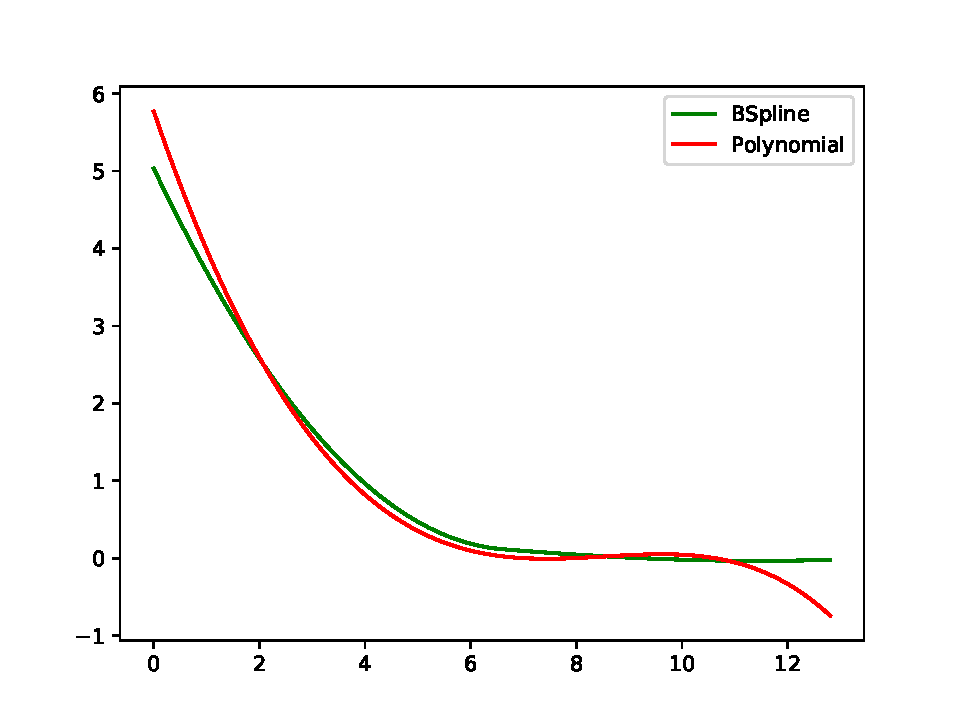
\includegraphics{ellipsoid.files/corr_fn.pdf}
\caption{BSpline vs.~Polynomail}
\end{figure}

\hypertarget{ellipsoid-method-revisited}{%
\section{Ellipsoid Method Revisited}\label{ellipsoid-method-revisited}}

\hypertarget{some-history-of-ellipsoid-method}{%
\subsection{Some History of Ellipsoid
Method}\label{some-history-of-ellipsoid-method}}

\begin{itemize}
\item
  Introduced by Shor and Yudin and Nemirovskii in 1976
\item
  Used to show that linear programming (LP) is polynomial-time solvable
  (Kachiyan 1979), settled the long-standing problem of determining the
  theoretical complexity of LP.
\item
  In practice, however, the simplex method runs much faster than the
  method, although its worst-case complexity is exponential.
\end{itemize}

\hypertarget{basic-ellipsoid-method}{%
\subsection{Basic Ellipsoid Method}\label{basic-ellipsoid-method}}

\begin{itemize}
\tightlist
\item
  An ellipsoid \(\mathcal{E}(x_c, P)\) is specified as a set
  \[\{x \mid (x-x_c)P^{-1}(x-x_c) \leq 1 \},\] where \(x_c\) is the
  center of the ellipsoid.
\end{itemize}

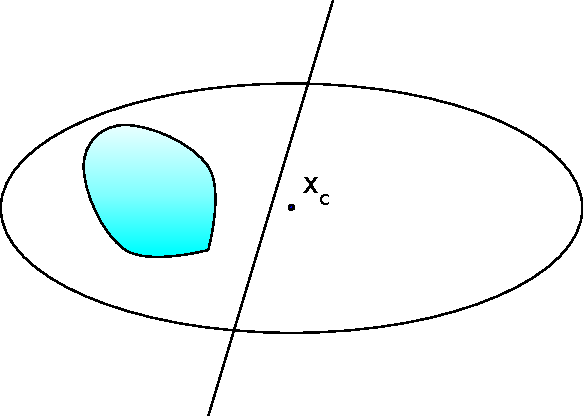
\includegraphics[width=0.9\textwidth,height=\textheight]{ellipsoid.files/ellipsoid.pdf}

\hypertarget{python-code-2}{%
\subsection{Python code}\label{python-code-2}}

\begin{lstlisting}[language=Python]
import numpy as np

class ell:
    def __init__(self, val, x):
        '''ell = { x | (x - xc)' * P^-1 * (x - xc) <= 1 }'''
        n = len(x)
        if np.isscalar(val):
            self.P = val * np.identity(n)
        else:
            self.P = np.diag(val)
        self.xc = np.array(x)
        self.c1 = float(n*n)/(n*n-1.)

    def update_core(self, calc_ell, cut):...
    def calc_cc(self, g):...
    def calc_dc(self, cut):...
    def calc_ll(self, cut):...
\end{lstlisting}

\hypertarget{updating-the-ellipsoid-deep-cut}{%
\subsection{Updating the ellipsoid
(deep-cut)}\label{updating-the-ellipsoid-deep-cut}}

\begin{itemize}
\tightlist
\item
  Calculation of minimum volume ellipsoid covering:
  \[\mathcal{E} \cap \{z \mid g^\top (z - x_c) + h \leq 0 \}\]
\item
  Let \(\tilde{g} = P\,g\), \(\tau^2 = g^\top P g\).
\item
  If \(n \cdot h < -\tau\) (shallow cut), no smaller ellipsoid can be
  found.
\item
  If \(h > \tau\), intersection is empty.
\item
  Otherwise, \[x_c^+ = x_c - \frac{\rho}{ \tau^2 } \tilde{g}, \qquad
  P^+ = \delta\cdot\left(P - \frac{\sigma}{ \tau^2 } \tilde{g}\tilde{g}^\top\right)\]
\end{itemize}

where \[\rho = \frac{ \tau+nh}{n+1}, \qquad
  \sigma = \frac{2\rho}{ \tau+h}, \qquad
  \delta = \frac{n^2(\tau^2 - h^2)}{(n^2 - 1)\tau^2}\]

\hypertarget{updating-the-ellipsoid-contd}{%
\subsection{Updating the ellipsoid
(cont'd)}\label{updating-the-ellipsoid-contd}}

\begin{itemize}
\tightlist
\item
  Even better, split \(P\) into two variables \(\kappa \cdot Q\)
\item
  Let \(\tilde{g} = Q \cdot g\), \(\omega = g^\top\tilde{g}\),
  \(\tau = \sqrt{\kappa\cdot\omega}\).
  \[x_c^+ = x_c - \frac{\rho}{\omega} \tilde{g}, \qquad
  Q^+ = Q - \frac{\sigma}{\omega} \tilde{g}\tilde{g}^\top, \qquad
  \kappa^+ =  \delta\cdot\kappa
   \]
\item
  Reduce \(n^2\) multiplications per iteration.
\item
  Note:

  \begin{itemize}
  \tightlist
  \item
    The determinant of \(Q\) decreases monotonically.
  \item
    The range of \(\delta\) is \((0, \frac{n^2}{n^2 - 1})\)
  \end{itemize}
\end{itemize}

\hypertarget{python-code-updating}{%
\subsection{Python code (updating)}\label{python-code-updating}}

\begin{lstlisting}[language=Python]
def update_core(self, calc_ell, cut):
    g, beta = cut
    Qg = self.Q.dot(g)
    omega = g.dot(Qg)
    tsq = self.kappa * omega
    if tsq <= 0.:
        return 4, 0.
    status, params = calc_ell(beta, tsq)
    if status != 0:
        return status, tsq
    rho, sigma, delta = params
    self._xc -= (rho / omega) * Qg
    self.Q -= (sigma / omega) * np.outer(Qg, Qg)
    self.kappa *= delta
    return status, tsq
\end{lstlisting}

\hypertarget{python-code-deep-cut}{%
\subsection{Python code (deep cut)}\label{python-code-deep-cut}}

\begin{lstlisting}[language=Python]
def calc_dc(self, beta, tsq):
    '''deep cut'''
    tau = math.sqrt(tsq)
    if beta > tau:
        return 1, None    # no sol'n
    if beta == 0.:
        return self.calc_cc(tau)
    n = self._n
    gamma = tau + n*beta
    if gamma < 0.:
        return 3, None  # no effect
    rho = gamma/(n + 1)
    sigma = 2.*rho/(tau + beta)
    delta = self.c1*(tsq - beta**2)/tsq
    return 0, (rho, sigma, delta)
\end{lstlisting}

\hypertarget{central-cut}{%
\subsection{Central Cut}\label{central-cut}}

\begin{itemize}
\tightlist
\item
  A Special case of deep cut when \(\beta = 0\)
\item
  Deserve a separate implement because it is much simplier.
\item
  Let \(\tilde{g} = Q\,g\), \(\tau = \sqrt{\kappa\cdot\omega}\),
\end{itemize}

\[\rho = {\tau \over n+1}, \qquad
  \sigma = {2 \over n+1}, \qquad
  \delta = {n^2 \over n^2 - 1}\]

\hypertarget{python-code-deep-cut-1}{%
\subsection{Python code (deep cut)}\label{python-code-deep-cut-1}}

\begin{lstlisting}[language=Python]
def calc_cc(self, tau):
    '''central cut'''
    np1 = self._n + 1
    sigma = 2. / np1
    rho = tau / np1
    delta = self.c1
    return 0, (rho, sigma, delta)
\end{lstlisting}

\hypertarget{parallel-cuts}{%
\section{Parallel Cuts}\label{parallel-cuts}}

\hypertarget{parallel-cuts-1}{%
\subsection{Parallel Cuts}\label{parallel-cuts-1}}

\begin{itemize}
\item
  Oracle returns a pair of cuts instead of just one.
\item
  The pair of cuts is given by \(g\) and \((\beta_1, \beta_2)\) such
  that: \[\begin{array}{l}
  g^\top (x - x_c) + \beta_1 \leq 0,  \\
  g^\top (x - x_c) + \beta_2 \geq 0,
  \end{array}\] for all \(x \in \mathcal{K}\).
\item
  Only linear inequality constraint can produce such parallel cut:
  \[ l \leq a^\top x + b \leq u, \qquad L \preceq F(x) \preceq U \]
\item
  Usually provide faster convergence.
\end{itemize}

\hypertarget{parallel-cuts-2}{%
\subsection{Parallel Cuts}\label{parallel-cuts-2}}

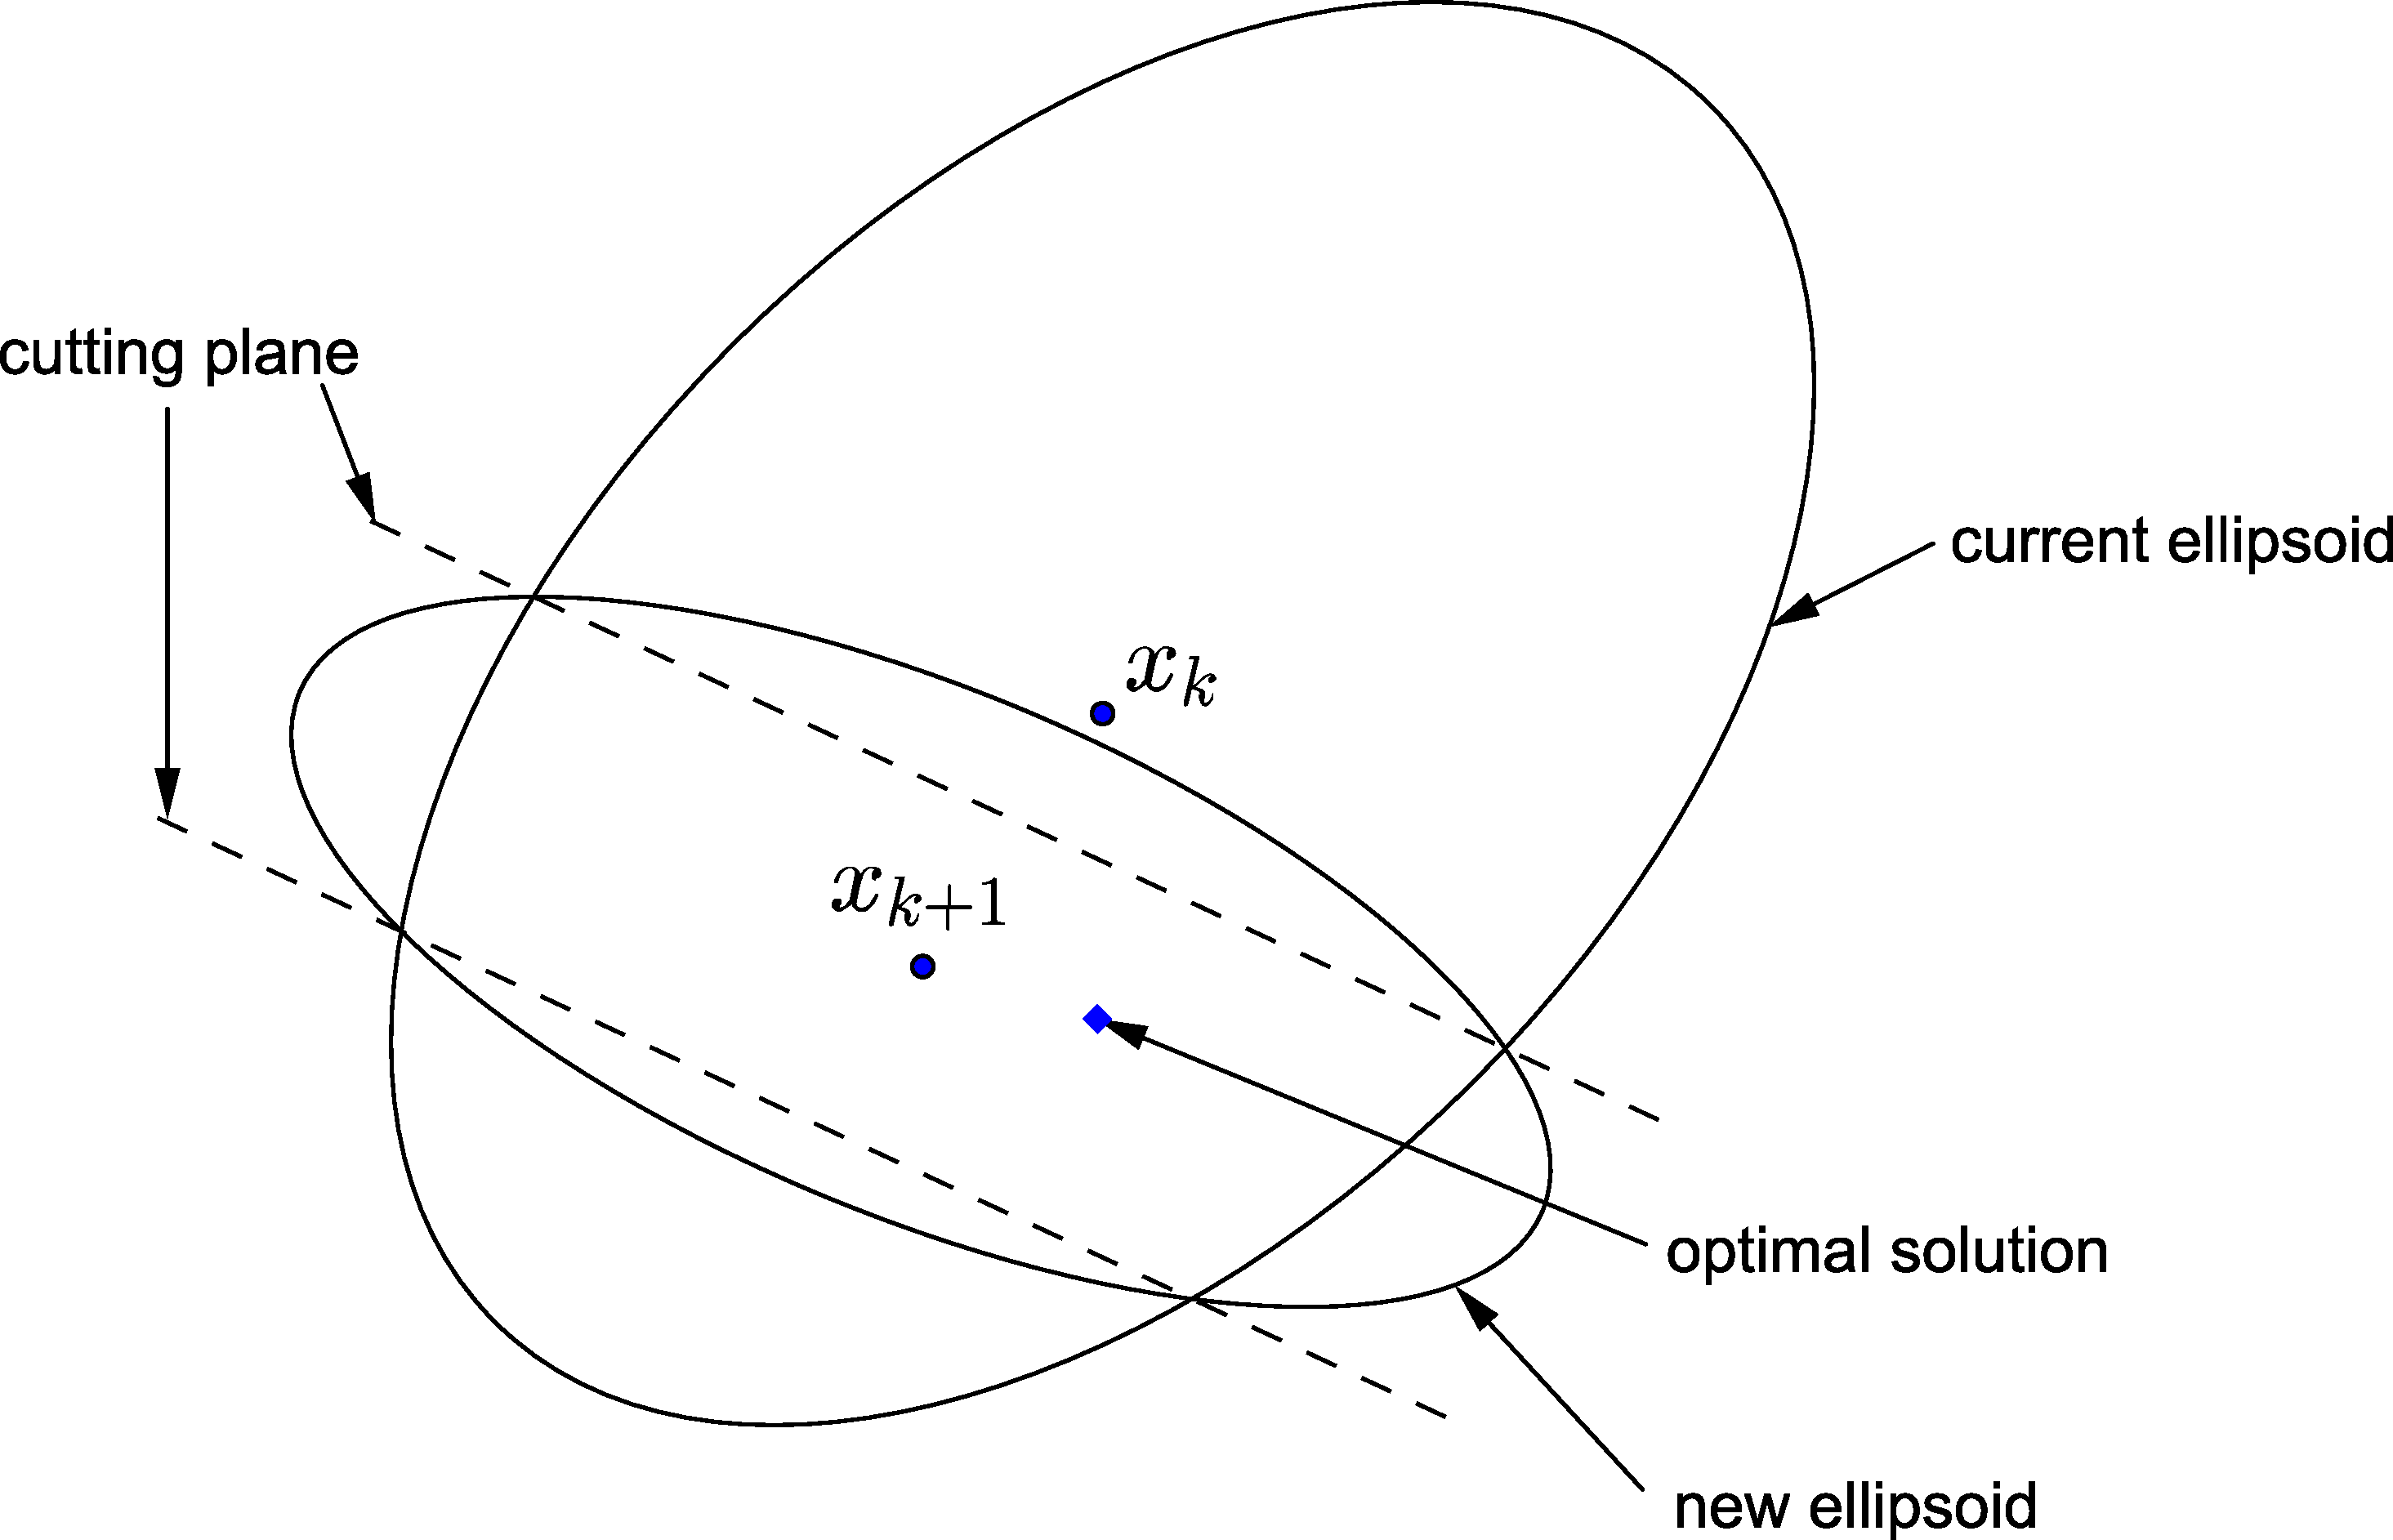
\includegraphics{ellipsoid.files/parallel_cut.pdf}

\hypertarget{updating-the-ellipsoid}{%
\subsection{Updating the ellipsoid}\label{updating-the-ellipsoid}}

\begin{itemize}
\item
  Let \(\tilde{g} = Q\,g\), \(\tau^2 = \kappa\cdot\omega\).
\item
  If \(\beta_1 > \beta_2\), intersection is empty.
\item
  If \(\beta_1 \beta_2 < -\tau^2/n\), no smaller ellipsoid can be found.
\item
  If \(\beta_2^2 > \tau^2\), it reduces to deep-cut with
  \(\alpha = \alpha_1\).
\item
  Otherwise, \[x_c^+ = x_c - \frac{\rho}{\omega} \tilde{g}, \qquad
  Q^+ = Q - \frac{\sigma}{\omega} \tilde{g}\tilde{g}^\top, \qquad
  \kappa^+ =  \delta \kappa
   \]

  where \[\begin{array}{lll}
    \bar{\beta} &=& (\beta_1 + \beta_2)/2 \\
    \xi^2 &=& (\tau^2 - \beta_1^2)(\tau^2 - \beta_2^2) + (n(\beta_2 - \beta_1)\bar{\beta})^2, \\
    \sigma &=& (n + (\tau^2 - \beta_1\beta_2 - \xi)/(2\bar{\beta}^2)) / (n + 1), \\
    \rho &=& \bar{\beta}\cdot\sigma, \\
    \delta &=& (n^2/(n^2-1)) (\tau^2 - (\beta_1^2 + \beta_2^2)/2 + \xi/n) / \tau^2
   \end{array}\]
\end{itemize}

\hypertarget{python-code-parallel-cut}{%
\subsection{Python code (parallel cut)}\label{python-code-parallel-cut}}

\scriptsize

\begin{lstlisting}[language=Python]
def calc_ll_core(self, b0, b1, tsq):
    if b1 < b0:
        return 1, None  # no sol'n
    n = self._n
    b0b1 = b0*b1
    if n*b0b1 < -tsq:
        return 3, None  # no effect
    b1sq = b1**2
    if b1sq > tsq or not self.use_parallel:
        return self.calc_dc(b0, tsq)
    if b0 == 0:
        return self.calc_ll_cc(b1, b1sq, tsq)
    # parallel cut
    t0 = tsq - b0**2
    t1 = tsq - b1sq
    bav = (b0 + b1)/2
    xi = math.sqrt( t0*t1 + (n*bav*(b1 - b0))**2 )
    sigma = (n + (tsq - b0b1 - xi)/(2 * bav**2)) / (n + 1)
    rho = sigma * bav
    delta = self.c1 * ((t0 + t1)/2 + xi/n) / tsq
    return 0, (rho, sigma, delta)
\end{lstlisting}

\hypertarget{example-fir-filter-design}{%
\subsection{Example: FIR filter
design}\label{example-fir-filter-design}}

\begin{figure}
\centering
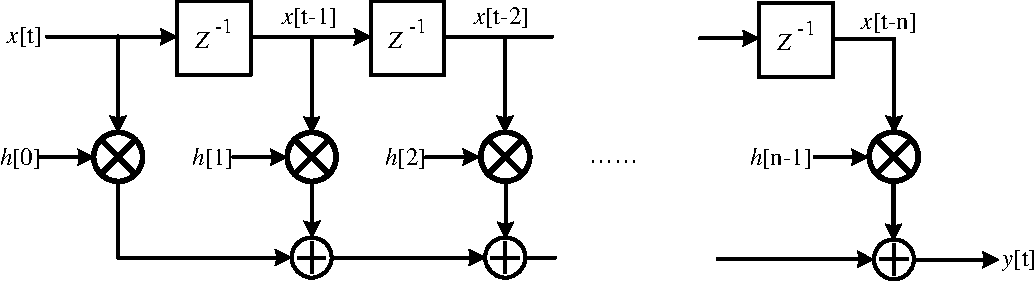
\includegraphics{ellipsoid.files/fir_strctr.pdf}
\caption{img}
\end{figure}

\begin{itemize}
\tightlist
\item
  The time response is: \[y[t] = \sum_{k=0}^{n-1}{h[k]u[t-k]}\]
\end{itemize}

\hypertarget{example-fir-filter-design-contd}{%
\subsection{Example: FIR filter design
(cont'd)}\label{example-fir-filter-design-contd}}

\begin{itemize}
\item
  The frequency response:
  \[H(\omega)~=~\sum_{m=0}^{n-1}{h(m)e^{-jm\omega}}\]
\item
  The magnitude constraints on frequency domain are expressed as

  \[L(\omega)~\leq~|H(\omega)|~\leq~U(\omega),~\forall~\omega\in(-\infty,+\infty)\]

  where \(L(\omega)\) and \(U(\omega)\) are the lower and upper
  (nonnegative) bounds at frequency \(\omega\) respectively.
\item
  The constraint is non-convex in general.
\end{itemize}

\hypertarget{example-fir-filter-design-contd-1}{%
\subsection{Example: FIR filter design
(cont'd)}\label{example-fir-filter-design-contd-1}}

\begin{itemize}
\tightlist
\item
  However, via \emph{spectral factorization}, it can transform into a
  convex one:
  \[L^2(\omega)~\leq~R(\omega)~\leq~U^2(\omega),~\forall~\omega\in(0,\pi)\]
  where

  \begin{itemize}
  \tightlist
  \item
    \(R(\omega)=\sum_{i=-1+n}^{n-1}{r(t)e^{-j{\omega}t}}=|H(\omega)|^2\)
  \item
    \(\mathbf{r}=(r(-n+1),r(-n+2),...,r(n-1))\) are the autocorrelation
    coefficients.
  \end{itemize}
\end{itemize}

\hypertarget{example-fir-filter-design-contd-2}{%
\subsection{Example: FIR filter design
(cont'd)}\label{example-fir-filter-design-contd-2}}

\begin{itemize}
\item
  \(\mathbf{r}\) can be determined by \(\mathbf{h}\):

  \[r(t)~=~\sum_{i=-n+1}^{n-1}{h(i)h(i+t)},~t\in\mathbf{Z}.\]

  where \(h(t)=0\) for \(t < 0\) or \(t > n - 1\).
\item
  The whole problem can be formulated as:
\end{itemize}

\[\begin{array}{ll}
  \text{min}  & \gamma \\
  \text{s.t.} & L^2(\omega) \leq R(\omega) \leq U^2(\omega), \; \forall \omega \in [0,\pi]   \\
              & R(\omega) > 0, \forall \omega \in [0,\pi]
\end{array}\]

\hypertarget{experiment}{%
\subsection{Experiment}\label{experiment}}

\begin{figure}
\centering
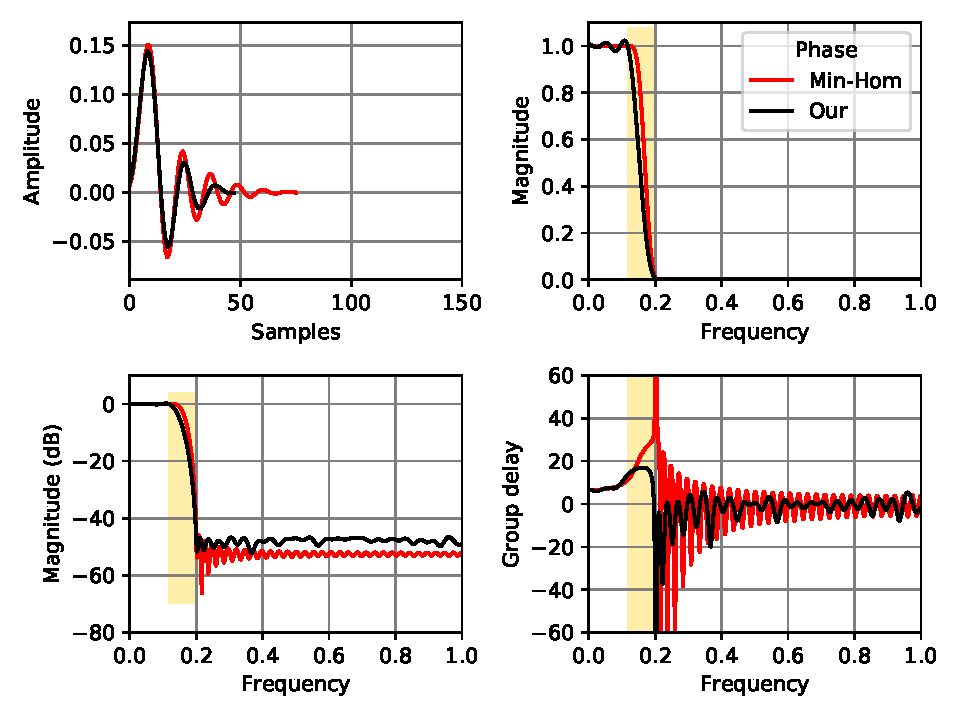
\includegraphics[width=0.5\textwidth,height=\textheight]{ellipsoid.files/lowpass.pdf}
\caption{Result}
\end{figure}

\hypertarget{example-maximum-likelihood-estimation}{%
\subsection{Example: Maximum Likelihood
estimation}\label{example-maximum-likelihood-estimation}}

\[\begin{array}{ll}
      \min_\kappa, p   &      \log \det (\Omega(p) + \kappa
       \cdot I) + \mathrm{Tr}((\Omega(p) + \kappa \cdot I)^{-1}Y) \\
      \text{s.t.} & \Omega(p) \succeq 0, \kappa \geq 0 \\
 \end{array}\]

Note: the 1st term is concave, the 2nd term is convex

\begin{itemize}
\tightlist
\item
  However, if there are enough samples such that \(Y\) is a positive
  definite matrix, then the function is convex within \([0, 2Y]\)
\end{itemize}

\hypertarget{example-maximum-likelihood-estimation-contd}{%
\subsection{Example: Maximum Likelihood estimation
(cont'd)}\label{example-maximum-likelihood-estimation-contd}}

\begin{itemize}
\tightlist
\item
  Therefore, the following problem is convex:
\end{itemize}

\[\begin{array}{ll}
      \min_\kappa, p   &   \log \det V(p) + \mathrm{Tr}(V(p)^{-1}Y) \\
      \text{s.t.} & \Omega(p) + \kappa \cdot I = V(p) \\
                    & 0 \preceq V(p) \preceq 2Y, \kappa {>} 0
\end{array}\]

\hypertarget{discrete-optimization}{%
\section{Discrete Optimization}\label{discrete-optimization}}

\hypertarget{why-discrete-convex-programming}{%
\subsection{Why Discrete Convex
Programming}\label{why-discrete-convex-programming}}

\begin{itemize}
\item
  Many engineering problems can be formulated as a convex/geometric
  programming, e.g.~digital circuit sizing
\item
  Yet in an ASIC design, often there is only a limited set of choices
  from the cell library. In other words, some design variables are
  discrete.
\item
  The discrete version can be formulated as a Mixed-Integer Convex
  programming (MICP) by mapping the design variables to integers.
\end{itemize}

\hypertarget{whats-wrong-w-existing-methods}{%
\subsection{What's Wrong w/ Existing
Methods?}\label{whats-wrong-w-existing-methods}}

\begin{itemize}
\item
  Mostly based on relaxation.
\item
  Then use the relaxed solution as a lower bound and use the
  branch--and--bound method for the discrete optimal solution.

  \begin{itemize}
  \tightlist
  \item
    Note: the branch-and-bound method does not utilize the convexity of
    the problem.
  \end{itemize}
\item
  What if I can only evaluate constraints on discrete data? Workaround:
  convex fitting?
\end{itemize}

\hypertarget{mixed-integer-convex-programming}{%
\subsection{Mixed-Integer Convex
Programming}\label{mixed-integer-convex-programming}}

Consider: \[\begin{array}{ll}
        \text{minimize}      & f_0(x), \\
        \text{subject to}    & f_j(x) \leq 0, \; \forall j=1,2,\ldots \\
                             & x \in \mathbb{D} 
\end{array}\]

where

\begin{itemize}
\tightlist
\item
  \(f_0(x)\) and \(f_j(x)\) are ``convex''
\item
  Some design variables are discrete.
\end{itemize}

\hypertarget{oracle-requirement}{%
\subsection{Oracle Requirement}\label{oracle-requirement}}

\begin{itemize}
\item
  The oracle looks for the nearby discrete solution \(x_d\) of \(x_c\)
  with the cutting-plane:
  \[g^\top (x - x_d) + \beta \leq 0, \beta \geq 0, g \neq 0\]
\item
  Note: the cut may be a shallow cut.
\item
  Suggestion: use different cuts as possible for each iteration (
  e.g.~round-robin the evaluation of constraints)
\end{itemize}

\hypertarget{example-fir-filter-design-1}{%
\subsection{Example: FIR filter
design}\label{example-fir-filter-design-1}}

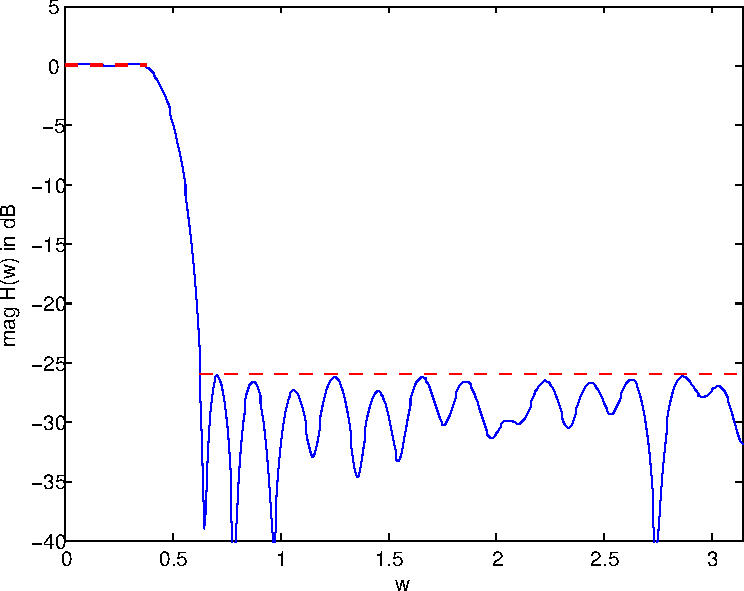
\includegraphics[width=0.9\textwidth,height=\textheight]{ellipsoid.files/lowpass_ripple.pdf}

\hypertarget{references}{%
\section*{References}\label{references}}
\addcontentsline{toc}{section}{References}

\end{document}
